\subsection{线段的和、差与画法}\label{subsec:czjh1-1-4}

我们学过数的加减运算,与数的加、减一样,两条线段也可以进行加、减, 得出新的线段。
一条线段的长度是另外两条线段长度的和(或差), 这条线段就是另两条线段的和(或差)。

如何画出两条线段的和或差呢?我们先学习下面的画法。

\liti 已知线段 $a$,画一条线段等于线段 $a$。

画一条线段等于已知线段有两种方法,一种是利用刻度尺来画;另一种是利用圆规和直尺来画。

\begin{figure}[htbp]
    \centering
    \begin{tikzpicture}
	\begin{scope}
		\tkzDefPoints{0/0/A, 2/0/B, 3/0/C,  -3/0/a, -1/0/b}
		\tkzDrawSegment[xianduan={below=0pt}](a,b)
		\tkzLabelSegment[above](a,b){$a$}
		\tkzDrawLine[add=0 and 0.1](A,C)
		\tkzLabelLine[pos=1.1,right=1em](A,C){甲}
		\tkzDrawSegment[xianduan={below=0pt}](A,B)
		\tkzDrawSegment[dim={$20$,-10pt,}](A,B)
		\tkzLabelPoints[above=0.3em](A,B,C)
	\end{scope}

	\begin{scope}[yshift=-1.5cm]
		\tkzDefPoints{0/0/A, 2/0/B, 3/0/C,  -3/0/a, -1/0/b}
		\tkzDrawSegment[xianduan={below=0pt}](a,b)
		\tkzLabelSegment[above](a,b){$a$}
		\tkzDrawLine[add=0 and 0.1](A,C)
		\tkzLabelLine[pos=1.1,right=1em](A,C){乙}
		\tkzDrawSegment[xianduan={below=0pt}](A,B)
		\tkzDrawSegment[dim={$a$,-10pt,}](A,B)
		\tkzLabelPoints[above=0.3em](A,B,C)
	\end{scope}
\end{tikzpicture}


    \caption{}\label{fig:czjh1-1-15}
\end{figure}

\huafa[1] 1. 用刻度尺量出线段的长度 20 mm (图 \ref{fig:czjh1-1-15} 甲)。

2. 画射线 $AC$。

3. 用刻度尺在射线 $AC$ 上取一点 $B$,使 $AB = 20 \;\haomi$。

线段 $AB$ 就是所求的线段。


\huafa[2] 1. 画射线 $AC$(图 \ref{fig:czjh1-1-15} 乙)。

2. 用圆规在射线 $AC$ 上截取 $AC = a$。

线段 $AB$ 就是所求的线段。


\liti 已知线段 $AB$ 与 $CD$, 且 $AB > CD$。 读下面的语句,并用圆规画图:

(1) 在线段 $AB$ 上取一点 $E$, 使 $AE = CD$;

(2) 延长线段 $AB$ 至点 $F$, 使 $BF = CD$。

\begin{figure}[htbp]
    \centering
    \begin{tikzpicture}
	\tkzDefPoints{0/0/A, 3/0/B, 2/0/E, 5/0/F,  -3/0/C, -1/0/D}
	\tkzDrawSegments[xianduan={below=0pt}](C,D  A,E  E,B  B,F)
	\tkzDrawLine[add=0 and 0.2](A,F)
	\tkzLabelPoints[above=0.3em](A,B,C,D,E,F)
\end{tikzpicture}


    \caption{}\label{fig:czjh1-1-16}
\end{figure}


\huafa (1) 用圆规在线段 $AB$上截取 $AE = CD$。点 $E$ 就是所求的点(图 \ref{fig:czjh1-1-16})。

(2) \begin{tblr}[t]{colsep=0pt, rowsep=0pt}
    1. 延长线段 $AB$。 \\
    2. 用圆规在 $AB$ 的延长线上截取 $BF = CD$。 点 $F$ 就是所求的点。
\end{tblr}

从以上的画图过程可知, $AE = CD$, $BF = CD$。所以
线段 $AF$ 的长度就是线段 $AB$ 的长度加线段 $CD$ 的长度;
线段 $BE$ 的长度就是线段 $AB$ 的长度减去线段 $CD$ 的长度。也就是说,
线段 $AF$ 是线段 $AB$ 与 $CD$ 的和,记作 $AF = AB + CD$;
线段 $BE$ 是线段 $AB$ 与 $CD$ 的差,记作 $BE = AB - CD$。

例 2 实际上就是线段的和与差的画法。

\begin{enhancedline}
如果一条线段 $b$ 是 $n$ 条线段 $a$ 的和,那么我们说线段 $b$ 是线段 $a$ 的 $n$倍,
或线段 $a$ 是线段 $b$ 的 $n$ 分之一。记作 $b = na$ 或 $a = \exdfrac{b}{n}$。

将一条线段分成两条相等线段的点,叫做\zhongdian{线段的中点}。
如图 \ref{fig:czjh1-1-17} , 点 $P$ 是线段 $EF$ 的中点.记作 $EP = PF$ 或 $EP = \exdfrac{1}{2}EF$。
\end{enhancedline}

\begin{figure}[htbp]
    \centering
    \begin{minipage}[b]{7cm}
        \centering
        \begin{tikzpicture}
	\tkzDefPoints{0/0/E, 3/0/F, 1.5/0/P}
	\tkzDrawSegments[xianduan={below=0pt}](E,P  P,F)
	\tkzLabelPoints[below](E,F,P)
\end{tikzpicture}


        \caption{}\label{fig:czjh1-1-17}
    \end{minipage}
    \qquad
    \begin{minipage}[b]{7cm}
        \centering
        \begin{tikzpicture}
	\tkzDefPoints{0/0/A, 1/0/B, 2/0/C, 3/0/D,  5/0/E, 0/1/a, 1/1/b}
	\tkzDrawSegment[xianduan={below=0pt}](a,b)
	\tkzLabelSegment[above](a,b){$a$}
	\tkzDrawLine[add=0 and 0.2](A,E)
	\tkzDrawSegments[xianduan={below=0pt}](A,B  B,C  C,D)
	\tkzDrawSegments[dim={$a$,-10pt,}](A,B  B,C  C,D)
	\tkzLabelPoints[above=0.3em](A,B,C,D,E)
\end{tikzpicture}


        \caption{}\label{fig:czjh1-1-18}
    \end{minipage}
\end{figure}


\liti 已知线段 $a$, 用直尺和圆规画一条线段,使它等于 $3a$。

\huafa 1. 画射线(图 \ref{fig:czjh1-1-18})。

2. 在射线 $AE$ 上,从点 $A$ 起顺次截取 $AB = BC = CD = a$。

线段 $AD$ 就是所求的线段。


\liti 已知线段 $a$、$b\; (a > b)$,画一条线段等于 $2a - b$。

\huafa 1. 画线段 $AB = 2a$(图 \ref{fig:czjh1-1-19})。

2. 在线段 $AB$ 上截取 $BC = b$。

线段 $AC$ 就是所求的线段。

\begin{figure}[htbp]
    \centering
    \begin{minipage}[b]{7cm}
        \centering
        \begin{tikzpicture}
	\tkzDefPoints{0/0/A, 4/0/B, 2.5/0/C, 2/0/M, 0/1/a, 2/1/b, 2.5/1/c, 4/1/d}
	\tkzDrawSegments[xianduan={below=0pt}](a,b  c,d)
	\tkzLabelSegment[above](a,b){$a$}
	\tkzLabelSegment[above](c,d){$b$}
	\tkzDrawLine[add=0 and 0.2](A,B)
	\tkzDrawSegments[xianduan={below=0pt}](A,M  C,B)
	\tkzDrawSegments[dim={$2a$,-2em,}](A,B)
	\tkzDrawSegments[dim={$b$,-1em,}](C,B)
	\tkzLabelPoints[above=0.3em](A,B,C)
\end{tikzpicture}


        \caption{}\label{fig:czjh1-1-19}
    \end{minipage}
    \qquad
    \begin{minipage}[b]{7cm}
        \centering
        \begin{tikzpicture}
	\tkzDefPoints{0/0/A, 2.4/0/B, 1.2/0/C}
	\tkzDrawSegments[xianduan={below=0pt}](A,B)

    % 将 1.2 cm 对应的箭头放在线段外侧
    % \tkzDrawSegments[dim={$1.2$cm,-1em,}](A,C)
    \tkzDefPoints{0/-0.3/a1, -0.3/-0.3/a2, 1.2/-0.3/c1, 1.5/-0.3/c2}
    \tkzDrawLine[add=0 and 0.5](C,c1)
    \tkzDrawSegments[-latex](a2,a1  c2,c1)
    \tkzLabelSegment[](A,C){\small $1.2$ cm}

	\tkzDrawSegments[dim={$2.4$ cm,-2em,}](A,B)
	\tkzLabelPoints[above=0.3em](A,B,C)
\end{tikzpicture}


        \caption{}\label{fig:czjh1-1-20}
    \end{minipage}
\end{figure}

\begin{enhancedline}
\liti 已知线段 $AB$。 画它的中点 $C$。

\huafa 用刻度尺量得 $AB = 2.4 \; \limi$, 计算得 $\exdfrac{1}{2} AB = \exdfrac{1}{2} \times 2.4 \; \limi = 1.2 \; \limi$(图 \ref{fig:czjh1-1-20})。

2. 在线段 $AB$ 上截取 $AC= 1.2\;\limi$。 点 $C$ 就是所求的中点。
\end{enhancedline}


\begin{lianxi}

\xiaoti{\footnotemark 已知线段 $AB$、$CD$。在线段 $AB$ 的延长线上取点 $G$,使 $BG = CD$;
    在线段 $AB$ 的反向延长线上取点 $K$, 使 $AK = BG$。
}
\footnotetext{本书第一、二章的画图题,做题时可不写画法,但要保留画图痕迹,并说朋结果。}


\xiaoti{已知线段 $a$、$b\; (a > b)$,用圆规和直尺画一条线段,使它等于 (1)$a + 2b$; (2) $3a - b$。}

\xiaoti{用刻度尺画一条线段 $AB = 5.4\;\limi$, 并把它三等分。}

\xiaoti{如图,已知直线 $l$ 上四点 $A$、$B$、$C$、$D$,根据图形填空:}
\begin{xiaoxiaotis}

    \xxt{$AD = \ewkh + \ewkh + \ewkh = AB + \ewkh = AC + \ewkh$;}

    \xxt{$BC = AC - \ewkh = \ewkh - CD = AD - \ewkh - \ewkh$。}

\end{xiaoxiaotis}

\begin{figure}[htbp]
    \centering
    \begin{tikzpicture}[scale=0.8]
	\tkzDefPoints{0/0/A, 2/0/B, 3/0/C,  5/0/D}
	\tkzDrawLine[add=0.1 and 0.3](A,D)
	\tkzLabelLine[pos=1.3,right=1em](A,D){$l$}
	\tkzDrawPoints[fill=black](A,B,C,D)
	\tkzLabelPoints[above](A,B,C,D)
\end{tikzpicture}


    \caption*{(第 4 题)}
\end{figure}

\end{lianxi}

